% ============================================================
%  Etapa4_1page.tex — Chapitre de thèse (1–2 pages)
%  Effet de la taille de dexel sur la croissance du chatter
% ============================================================
\documentclass[11pt,a4paper]{article}

% ── Géométrie ────────────────────────────────────────────────
\usepackage[top=2.0cm, bottom=2.0cm, left=2.0cm, right=2.0cm]{geometry}

% ── Encodage / langue ────────────────────────────────────────
\usepackage[utf8]{inputenc}
\usepackage[T1]{fontenc}
\usepackage[french]{babel}
\usepackage{csquotes}
\usepackage{microtype}
\usepackage{lmodern}

% ── Maths ────────────────────────────────────────────────────
\usepackage{amsmath, amssymb}
\usepackage{siunitx}
\sisetup{output-decimal-marker={,}, locale=FR}

% ── Figures ──────────────────────────────────────────────────
\usepackage{graphicx}
\usepackage{float}
\usepackage{subcaption}

% ── Mise en page ─────────────────────────────────────────────
\usepackage{setspace}
\setstretch{1.10}
\setlength{\parindent}{0pt}
\setlength{\parskip}{0.5em}

% ── Sections ─────────────────────────────────────────────────
\usepackage{titlesec}
\titlespacing*{\section}{0pt}{8pt}{4pt}
\titlespacing*{\subsection}{0pt}{5pt}{2pt}
\titleformat{\section}{\normalfont\bfseries\large}{\thesection.}{0.5em}{}
\titleformat{\subsection}{\normalfont\bfseries\normalsize}{\thesubsection.}{0.5em}{}

% ── Hyperref ─────────────────────────────────────────────────
\usepackage[hidelinks]{hyperref}

% ── Macros ───────────────────────────────────────────────────
\newcommand{\ap}{a_p}
\newcommand{\apz}{a_{p,0}}
\newcommand{\apf}{a_{p,1}}
\newcommand{\apcrit}{a_{p,\mathrm{crit}}}
\newcommand{\trampe}{t_{\mathrm{rampe}}}
\newcommand{\dxli}{h_{d,i}}
\newcommand{\omn}{\omega_n}
\newcommand{\omnsq}{\omega_n^{2}}
\newcommand{\dFin}{\delta F_{i,\mathrm{n}}}
\newcommand{\Ri}{R_i(t)}
\newcommand{\betai}{\beta_i}
\newcommand{\cfit}{c_i^{\mathrm{fit}}}
\newcommand{\Qi}{Q_i^{2}}
\newcommand{\Pproxy}{P_{h,i}}
\newcommand{\cFi}{c_i^{F}}
\newcommand{\Aref}{A_{\mathrm{ref}}}
\newcommand{\tfit}{t_i^{\mathrm{fit}}}
\newcommand{\tF}{t_i^{F}}
\newcommand{\Dtfit}{\Delta t_{ij}^{\mathrm{fit}}}
\newcommand{\DtF}{\Delta t_{ij}^{F}}
\newcommand{\DtPfit}{\Delta t_{P,ij}^{\mathrm{fit}}}
\newcommand{\DtPF}{\Delta t_{P,ij}^{F}}
\newcommand{\Dtbfit}{\Delta t_{\beta,ij}^{\mathrm{fit}}}
\newcommand{\DtbF}{\Delta t_{\beta,ij}^{F}}
\newcommand{\RMS}{\operatorname{RMS}}
\newcommand{\lmax}{\lambda_{\max}}
\newcommand{\betath}{\beta_{\mathrm{th}}}
\newcommand{\Kf}{K_f}

% ============================================================
\begin{document}

% ── Titre ────────────────────────────────────────────────────
\begin{center}
  {\large\bfseries
    Effet de la taille de dexel sur la croissance du chatter :\\
    extraction de $\betai$, proxy de perturbation et décomposition du décalage temporel}\\[4pt]
\end{center}
\hrule
% \vspace{6pt}

% =========================================================
\section{Observation et contexte}
% =========================================================

Les simulations de usinage sur le cône tronqué sont réalisées pour différentes valeurs de
taille de dexel $\dxli$, avec une profondeur de coupe croissant linéairement de
$\apz = \SI{5}{\milli\metre}$ à $\apf = \SI{15}{\milli\metre}$ sur la durée
$\trampe$. Le système traverse ainsi un seuil de stabilité $\apcrit$ et entre en
régime de chatter. L'observation centrale est la suivante : lorsque $\dxli$
diminue, le début de la croissance exponentielle est systématiquement décalé vers
des temps plus élevés. Ce retard peut avoir deux origines non exclusives.
\textbf{Premièrement}, la discrétisation introduit une erreur géométrique sur la
surface usinée, ce qui se traduit par une perturbation initiale d'autant plus
faible que $\dxli$ est petit ; le signal démarre donc à un niveau plus bas et met
plus de temps à atteindre un niveau donné.
\textbf{Deuxièmement}, la représentation de l'épaisseur instantanée de coupe
peut modifier le couplage régénératif et donc le taux de croissance $\betai$.


% =========================================================
\section{Extraction du taux de croissance \texorpdfstring{$\betai$}{beta i}}
% =========================================================

\subsection{RMS glissant et ajustement log-linéaire}

La dynamique de l'outil est régie par l'équation régénérative
$m\ddot{x} + c\dot{x} + kx = \Kf\ap(t)[x(t-T)-x(t)]$.
La force résiduelle normalisée $\dFin = \delta F_i / \ap(t) \approx \Kf[x_i(t-T)-x_i(t)]$
isole la contribution dynamique pure en supprimant la tendance croissante liée à
la rampe. L'amplitude instantanée est estimée par l'enveloppe RMS sur une fenêtre
glissante $T_w = 5/f_n$ :
\[
  R_i(t) = \sqrt{\frac{1}{T_w}\int_{t-T_w/2}^{t+T_w/2} \dFin(\tau)^2 \, d\tau}.
\]
Dans la zone instable, $R_i(t)$ suit une croissance exponentielle. Un ajustement
log-linéaire sur l'intervalle $I_i = [t_{a,i},\, t_{b,i}]$ donne
\begin{equation}\label{eq:logfit}
  \ln R_i(t) = \betai\, t + \cfit, \qquad t \in I_i,
\end{equation}
où $\betai$ est la pente (taux de croissance numérique) et $\cfit = \ln P_i^{\mathrm{fit}}$
est l'ordonnée à l'origine. 

% La qualité de l'ajustement est mesurée par $\Qi \approx 1$.
\vspace{-0.25cm}
\begin{figure}[H]
  \centering
  \begin{subfigure}[t]{0.49\textwidth}
    \centering
    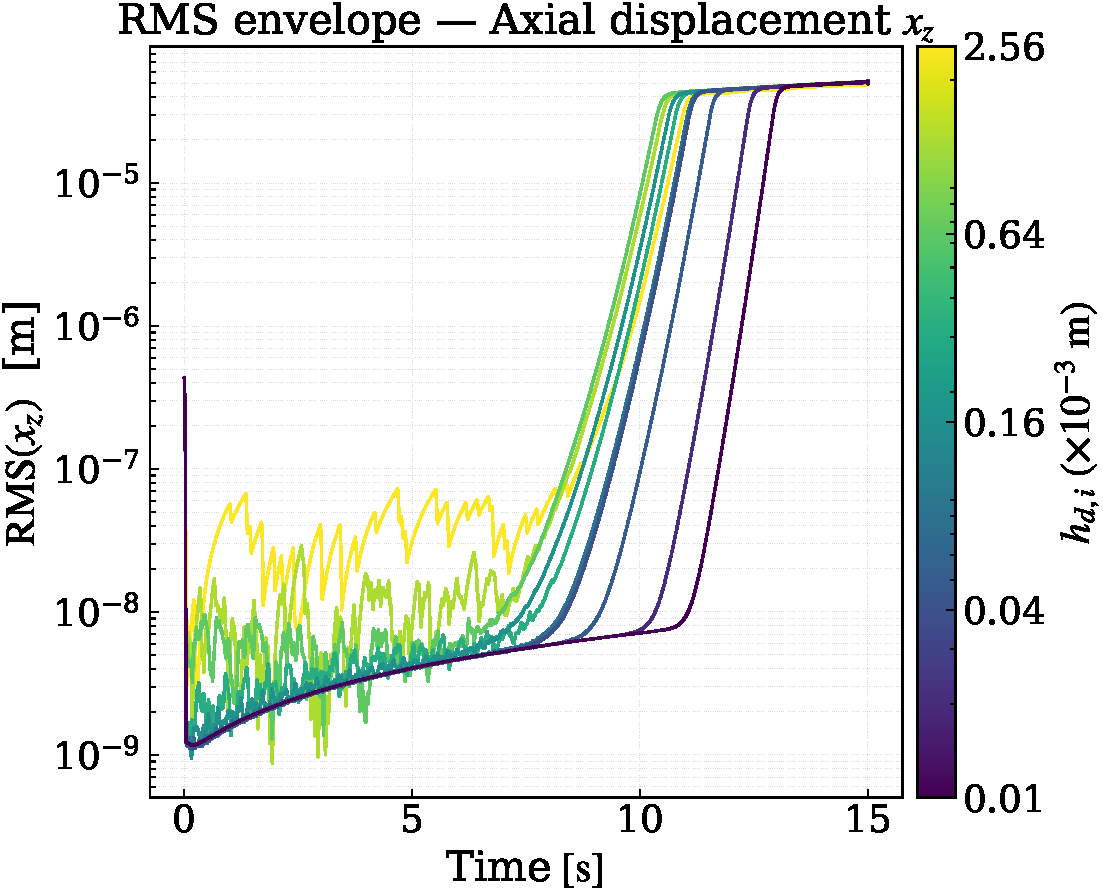
\includegraphics[width=\linewidth]{Images/lnRMS_Axial_disp.pdf}
    \caption{Enveloppes $\ln R_i(t)$ du déplacement axial.}
    \label{fig:lnR-disp}
  \end{subfigure}
  \hfill
  \begin{subfigure}[t]{0.49\textwidth}
    \centering
    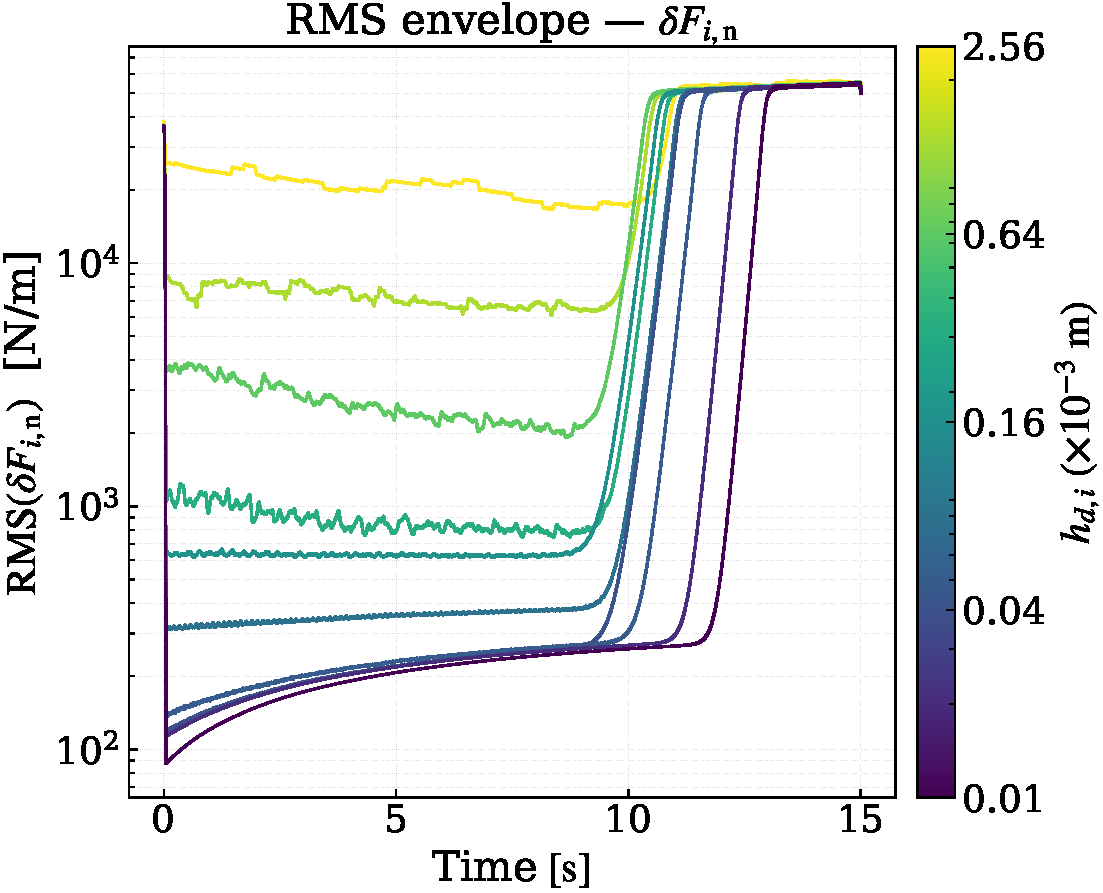
\includegraphics[width=\linewidth]{Images/lnRMS_dF_norm.pdf}
    \caption{Enveloppes $\ln R_i(t)$ de la force résiduelle normalisée.}
    \label{fig:lnR-dFnorm}
  \end{subfigure}
  \caption{Enveloppes RMS log-linéaires pour les $N$ cas de discrétisation.}
  \label{fig:lnR-Aref}
\end{figure}




\subsection{Comparaison avec le taux théorique}

À chaque instant $t_k$, on gèle $\ap(t_k)$ et on résout l'équation caractéristique
du système retardé :
\begin{equation}\label{eq:char}
  m\lambda^2 + c\lambda + k + \Kf\,\ap(t_k)\bigl(1 - e^{-\lambda T}\bigr) = 0.
\end{equation}
Le taux théorique est la partie réelle de la valeur propre dominante,
$\betath(t_k) = \operatorname{Re}\{\lmax[\ap(t_k)]\}$.
Il est négatif en zone stable, nul au seuil $\apcrit$ et positif dans la zone
instable. La figure~\ref{fig:beta-comparison} superpose $\betath(t)$ aux taux
numériques $\betai$ : les taux extraits de la simulation augmentent avec $\dxli$,
car un dexel plus grand surestime l'épaisseur instantanée de coupe, ce qui
amplifie le couplage régénératif.

% La qualité de l'ajustement est mesurée par $\Qi \approx 1$.
\vspace{-0.0cm}
\begin{figure}[H]  
  \begin{subfigure}[t]{0.49\textwidth}
    \centering
    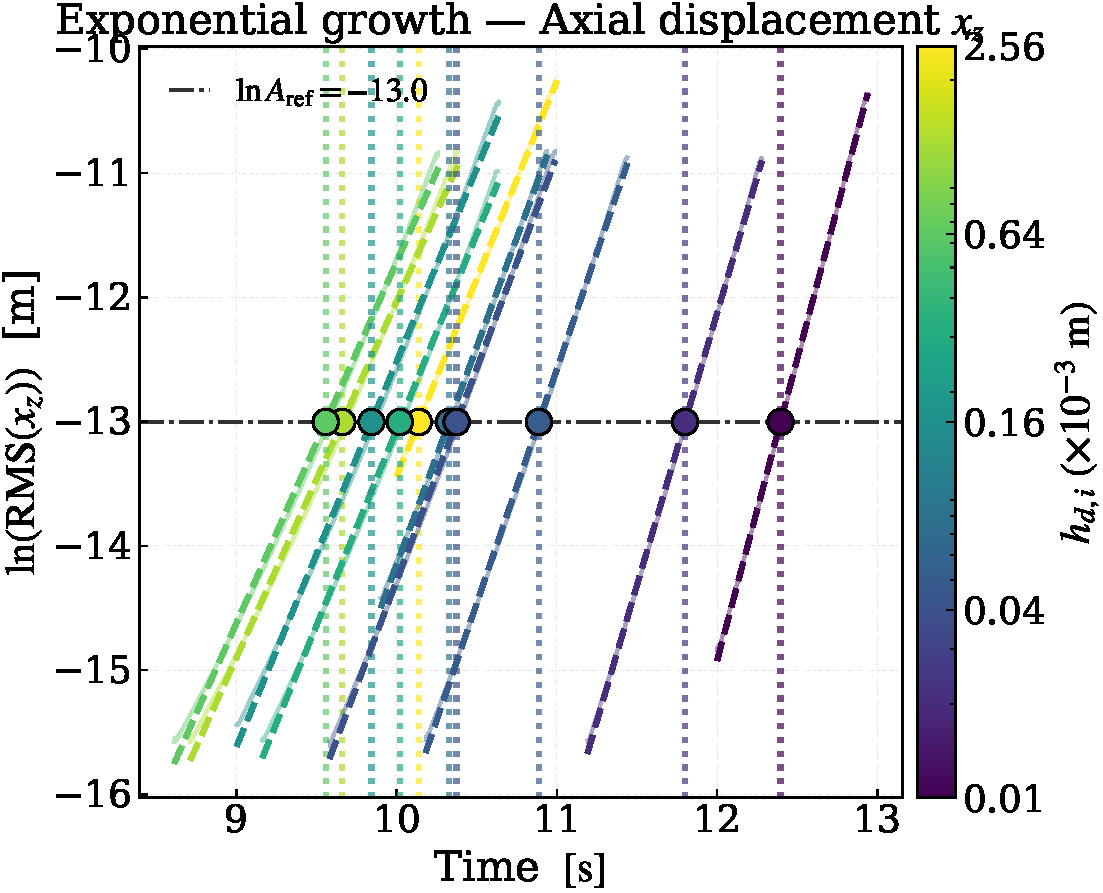
\includegraphics[width=\linewidth]{Images/lnRMS_fits_Axial_disp.pdf}
    \caption{Ajustement log-linéair
    }
    \label{fig:lnR-fits}
  \end{subfigure}
  \hfill
  \centering
  \begin{subfigure}[t]{0.49\textwidth}
    \centering
    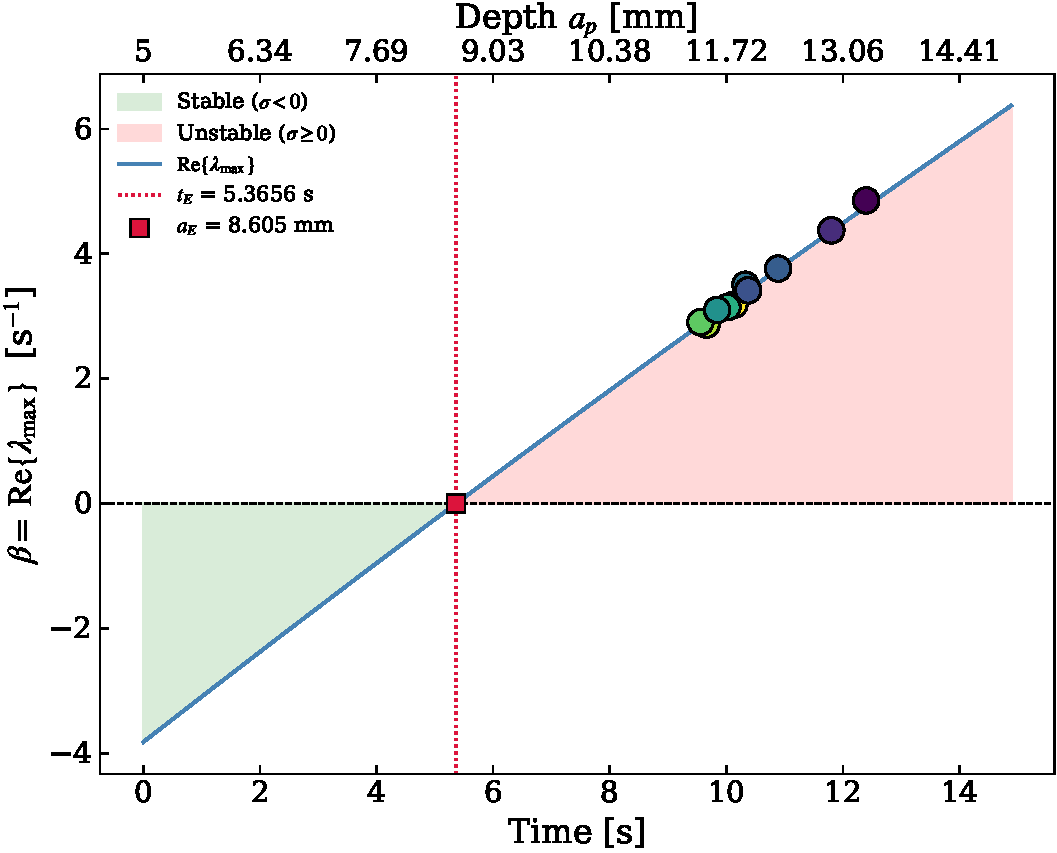
\includegraphics[width=\linewidth]{Images/stability_betas_Axial_disp.pdf}
    \caption{Taux de croissance théorique $\betath$ et des taux numériques $\betai$.}
    \label{subfig:beta-comparison}
  \end{subfigure}


  \caption{ Ajustement log-linéaire dans l'intervalle $I_i = [t_{a,i},\, t_{b,i}]$, niveau de référence $\Aref$ et  $t_i^{\mathrm{mes}}$ (mesuré directement).Comparaison du taux de croissance théorique $\betath$ et des taux numériques $\betai$ en fonction du temps et de la profondeur de coupe instantanée.}
  \label{fig:beta-comparison}
\end{figure}


% =========================================================
\section{Trois estimateurs du décalage temporel}
% =========================================================

\subsection{Niveau de référence et estimateurs par ajustement et mesure directe}

On choisit un niveau commun $\Aref$ atteint par toutes les courbes $R_i(t)$ dans
leurs intervalles $I_i$. Trois estimateurs indépendants du décalage $\Dtfit$
entre les cas $i$ et $j$ sont définis.

\textbf{Estimateur mesuré.} Le temps $t_i^{\mathrm{mes}}$ est le premier instant
où la courbe RMS réelle atteint $\Aref$, lu directement sur le signal sans
ajustement. Le décalage est $\Delta t_{ij}^{\mathrm{mes}} = t_j^{\mathrm{mes}} - t_i^{\mathrm{mes}}$.

\textbf{Estimateur par ajustement.} À partir du modèle~\eqref{eq:logfit}, on
extrapole le temps d'atteinte de $\Aref$ :
\[
  \tfit = \frac{\ln\Aref - \cfit}{\betai}, \qquad \Dtfit = t_j^{\mathrm{fit}} - \tfit.
\]
Cet estimateur filtre le bruit via la régression log-linéaire et est utilisé
comme référence pour la décomposition analytique.

\subsection{Proxy de force — troisième estimateur avec correction temporelle}

La taille de dexel ne s'observe pas directement, mais $\dFin(t)$ est
proportionnelle à $\Kf[x_i(t-T)-x_i(t)]$, qui dépend de l'erreur géométrique
introduite par la discrétisation. On évalue son RMS local à l'instant $t_{s,i}$
(début de la fenêtre d'ajustement) pour obtenir le \textbf{proxy de perturbation}
$\Pproxy$. Ce proxy est évalué à un instant différent pour chaque cas ; il faut
donc corriger cet écart temporel avant de comparer les amplitudes.

% Pour un signal
% exponentiel sinusoïdal d'enveloppe $e^{\betai t}$, le facteur de
% proportionnalité entre $\RMS[\dFin]$ et $\RMS[x_i]$ est analytiquement :
% \[
%   C_i = \sqrt{1 + e^{-2\betai T} - 2\,e^{-\betai T}\cos(\omega_i T)}
%   \;\approx\; 2\left|\sin\!\tfrac{\omega_i T}{2}\right| \quad (\betai T \ll 1).
% \]


% En ramenant $\Pproxy$ à $t=0$ via la correction $e^{-\betai t_{s,i}}$ et en
% tenant compte de $\Kf$ et $C_i$, l'ordonnée à l'origine reconstruite est

En ramenant $\Pproxy$ à $t=0$ via la correction $e^{-\betai t_{s,i}}$, l'ordonnée à l'origine reconstruite est
$\cFi = \ln\Pproxy - \ln\Kf - \ln C_i - \betai\,t_{s,i}$,
et le temps d'atteinte de $\Aref$ est
\begin{equation}\label{eq:tF}
  \tF = \frac{\ln\Aref - \cFi}{\betai}
      = t_{s,i} + \frac{1}{\betai}\ln\!\left(\frac{\Kf C_i \Aref}{\Pproxy}\right),
  \qquad \DtF = t_j^F - \tF.
\end{equation}
% La cohérence $\Delta t^{\mathrm{mes}} \approx \Dtfit \approx \DtF$ constitue
% le critère de validation de la méthode.

% =========================================================
\section{Décomposition analytique du décalage \texorpdfstring{($\betai \neq \beta_j$)}{beta i != beta j}}
% =========================================================

Dans le cas général où $\betai \neq \beta_j$, les deux estimateurs se
décomposent en deux contributions indépendantes.

\textbf{Décomposition de $\Dtfit$ (ajustement) :}
\begin{equation}\label{eq:decomp-fit}
  \Dtfit
  = \underbrace{\frac{1}{\beta_j}\ln\!\left(\frac{P_i^{\mathrm{fit}}}{P_j^{\mathrm{fit}}}\right)}_{\DtPfit
    \;(\text{perturbations initiales})}
  +\; \underbrace{\ln\!\left(\frac{\Aref}{P_i^{\mathrm{fit}}}\right)
    \!\left(\frac{1}{\beta_j} - \frac{1}{\betai}\right)}_{\Dtbfit
    \;(\text{taux de croissance})}.
\end{equation}

\textbf{Décomposition de $\DtF$ (proxy de force) :}
\begin{equation}\label{eq:decomp-force}
  \DtF
  = \underbrace{\frac{1}{\beta_j}\ln\!\left(\frac{\Pproxy\,C_j}{P_{h,j}\,C_i}\right)
    - \frac{\betai}{\beta_j}t_{s,i} + t_{s,j}}_{\DtPF
    \;(\text{perturbations initiales})}
  +\; \underbrace{(\ln\Aref - \ln\Pproxy + \ln\Kf + \ln C_i + \betai\,t_{s,i})
    \!\left(\frac{1}{\beta_j} - \frac{1}{\betai}\right)}_{\DtbF
    \;(\text{taux de croissance})}.
\end{equation}

$\DtPfit$ (resp.\ $\DtPF$) est le décalage dû aux niveaux initiaux différents
à $\beta$ égal ; il converge vers zéro quand les deux cas ont la même
perturbation. $\Dtbfit$ (resp.\ $\DtbF$) est nul si et seulement si
$\betai = \beta_j$ et dépend de $\Aref$. 

La vérification numérique
$\Dtfit = \DtPfit + \Dtbfit$ (et idem pour $\DtF$) valide la décomposition.



\begin{figure}[H]
  \centering
  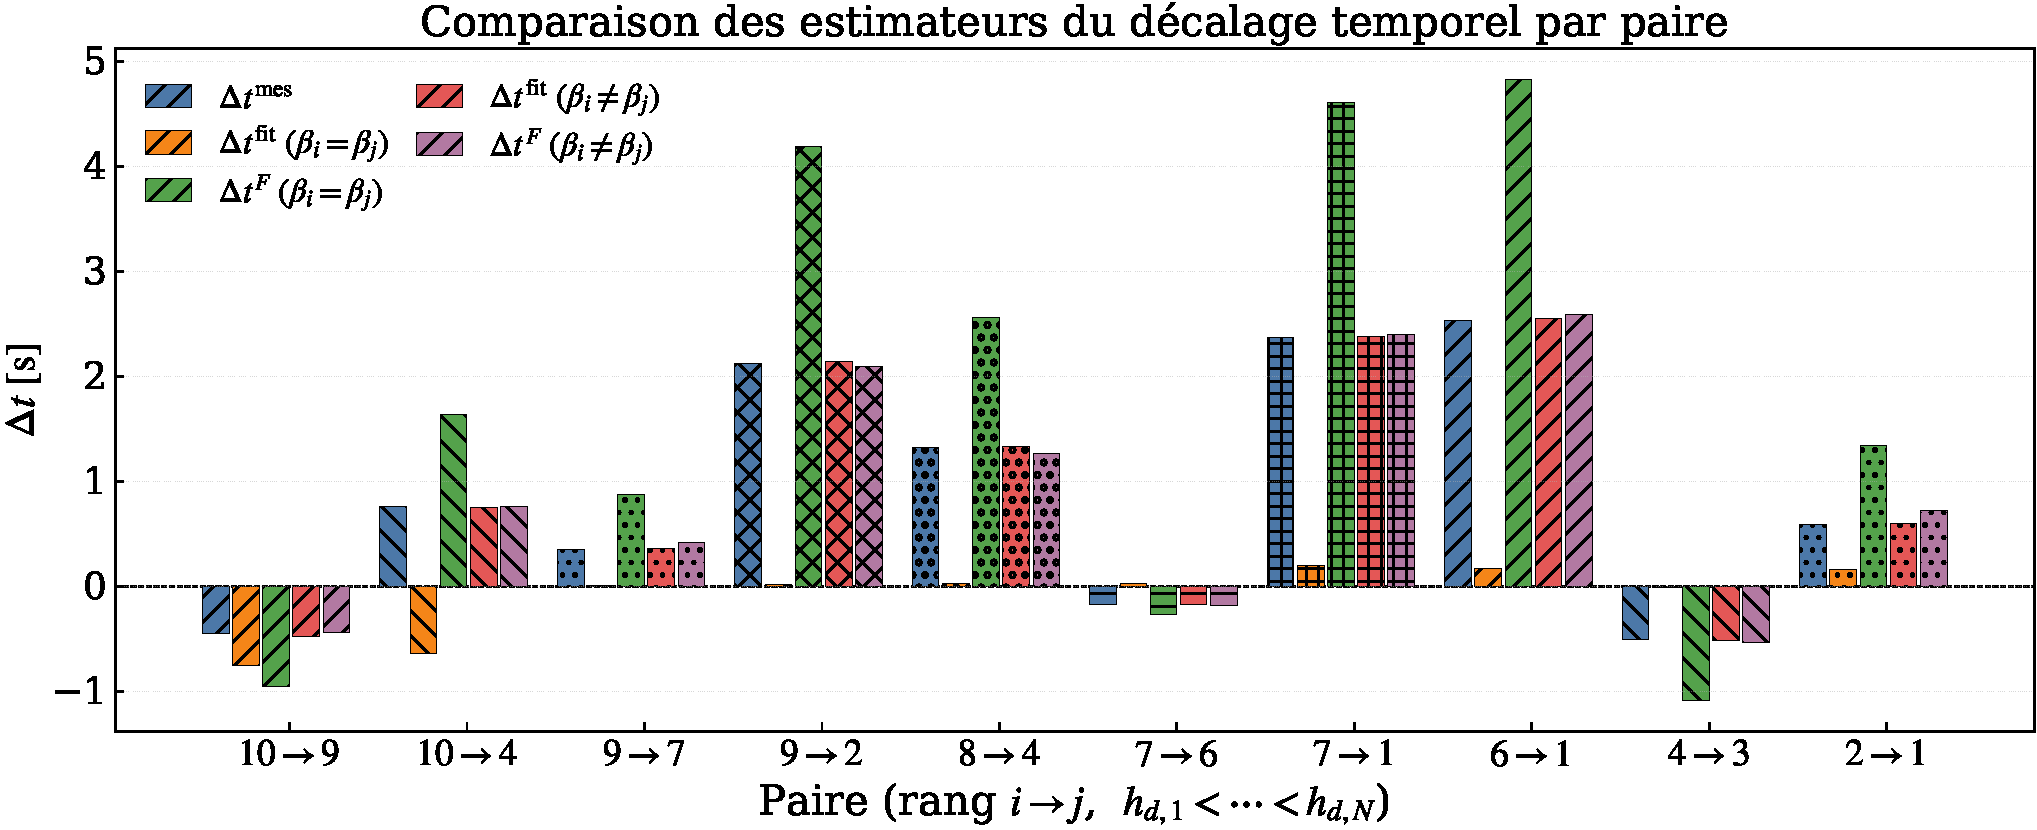
\includegraphics[width=0.99\linewidth]{Images/delta_t_bars_Axial_disp.pdf}
  \caption{Comparaison des estimateurs du décalage temporel et décomposition
           en contributions de niveau initial ($\Delta t_P$) et de taux de
           croissance ($\Delta t_\beta$), pour chaque paire de cas.}
  \label{fig:barres-decomp}
\end{figure}

La figure~\ref{fig:barres-decomp} compare, pour des paires de cas représentatives $(i,j)$, des
estimateurs de $\Delta t$ : la mesure directe $\Delta t^{\mathrm{mes}}$ (bleu),
l'ajustement log-linéaire sous l'hypothèse $\betai=\beta_j$ (orange), le proxy de
perturbation sous la même hypothèse (vert), et leurs analogues à $\betai\neq\beta_j$
(rouge et violet, respectivement). Deux observations se dégagent.
\textbf{Premièrement}, les estimateurs à betas différents (rouge et violet) sont
systématiquement plus proches de la mesure directe que leurs homologues à betas
égaux, ce qui confirme que l'écart de taux de croissance $\betai-\beta_j$ n'est
pas négligeable et doit être pris en compte dans la décomposition.
\textbf{Deuxièmement}, le proxy de perturbation à betas différents (violet) est
très proche des deux autres estimateurs précis, ce qui valide que la variation de
$\dxli$ agit principalement via la perturbation initiale : un dexel plus fin génère
un niveau de départ plus faible, retardant l'entrée en régime exponentiel.




\vspace{6pt}\hrule\vspace{4pt}
{\small\textit{Notas Completas Revisar : \texttt{Etapa4.tex} (notes) — \texttt{Etapa4\_article.tex} (article).}}

\end{document}
